% ===================================================================== 
%  ICOKG 2026 -- Paper 37 -- CAMERA-READY
%  Springer ACSAR (Advances in Computer Science Applications and Research)
%  Springer LNCS class (llncs.cls v2.22)
%
%  PDF CON LOS CAMBIOS MARCADOS:
%     python scripts/marcar_cambios.py
%  Compara este fichero contra el que se envio a revision y escribe
%  paper/main_with_changes.pdf con lo anadido en azul subrayado y lo
%  suprimido en rojo tachado. Las marcas se derivan de la comparacion,
%  no de envoltorios puestos a mano.
% ===================================================================== 

\documentclass[runningheads]{llncs}

% --- Fonts -----------------------------------------------------------
% NOTE: the reviewed PDF embedded Type 3 (bitmap) fonts, which breaks
% copy/paste, in-PDF search, indexing and Springer's PDF checks.
% Cause: [T1]{fontenc} without lmodern/cm-super installed.
% Fix: load a Type 1 Times family (also the font family requested by ACSAR).
\usepackage[T1]{fontenc}
\usepackage[utf8]{inputenc}
\usepackage{mathptmx}
\usepackage[scaled=.90]{helvet}
\usepackage{courier}
\input{glyphtounicode}\pdfgentounicode=1

\usepackage[english]{babel}
\usepackage{graphicx}
\usepackage{booktabs}
\usepackage{url}
\usepackage{amsmath}
\usepackage{amssymb}
\usepackage{array}
\usepackage{xcolor}
\usepackage{tikz}
\usetikzlibrary{arrows.meta,positioning,shapes.geometric,fit,backgrounds,calc}
\usepackage{hyperref}

% --- Revision marks --------------------------------------------------

% --- Tighter bibliography spacing -------------------------------------
% Sin cambiar el cuerpo de texto ni el estilo LNCS: sólo se elimina el
% espacio suelto entre entradas, que con once referencias costaba media
% página y dejaba el capítulo por encima del límite.
\let\origthebibliography\thebibliography
\renewcommand{\thebibliography}[1]{%
  \origthebibliography{#1}%
  \setlength{\itemsep}{0pt}\setlength{\parsep}{0pt}\setlength{\parskip}{0pt}}

% --- Line breaks in underscore identifiers ---------------------------
\let\origunderscore\_
\renewcommand{\_}{\origunderscore\allowbreak}
\emergencystretch=3em
\linespread{0.94}\selectfont

% --- tighter float spacing (keeps the paper inside the page budget) ---
\setlength{\textfloatsep}{10pt plus 2pt minus 2pt}
\setlength{\floatsep}{8pt plus 2pt minus 2pt}
\setlength{\intextsep}{8pt plus 2pt minus 2pt}
\setcounter{topnumber}{3}\setcounter{bottomnumber}{2}\setcounter{totalnumber}{4}
\renewcommand{\topfraction}{0.9}\renewcommand{\bottomfraction}{0.7}
\renewcommand{\textfraction}{0.08}\renewcommand{\floatpagefraction}{0.8}

% Mismo tratamiento de enlaces que el capítulo del almacén de agua enviado
% a ICOKG 2026: un solo azul para enlaces internos, URLs y citas. Antes las
% URLs y los ORCID salían en cian, que no coincidía con aquel formato.
\renewcommand\UrlFont{\rmfamily}
\hypersetup{colorlinks=true,linkcolor=blue,urlcolor=blue,citecolor=blue}
\def\UrlBreaks{\do\/\do-\do_\do.}

\begin{document}

\title{A Dimensional Data Warehouse for Geospatial Monitoring of
Municipal Public Works, with an Evolution Path Toward a Lakehouse Architecture}
\titlerunning{Data Warehouse for Geospatial Monitoring of Public Works}

\author{%
Uriel Gonz\'alez Casiano\href{https://orcid.org/0009-0009-8172-9584}{\orcidID{0009-0009-8172-9584}} \and
Marco Tulio Maldonado Mej\'ia\href{https://orcid.org/0009-0005-4691-9607}{\orcidID{0009-0005-4691-9607}} \and
Gabriel Hurtado Avil\'es\thanks{Corresponding author: \href{mailto:gabrielhuav@gmail.com}{gabrielhuav@gmail.com}}\href{https://orcid.org/0009-0002-5686-1822}{\orcidID{0009-0002-5686-1822}}}

\authorrunning{U. Gonz\'alez Casiano et al.}

\institute{Escuela Superior de C\'omputo (ESCOM), Instituto Polit\'ecnico Nacional, Mexico City, Mexico\\
\email{\{ugonzalezc2400,mmaldonadom2200\}@alumno.ipn.mx}\\
\email{ghurtadoa@ipn.mx}\\
\email{gonzalezcasianouriel@gmail.com, marcotuliomm.s45@gmail.com, gabrielhuav@gmail.com}}

\maketitle

\begin{abstract}
The accelerated growth of public infrastructure data in municipal governments generates heterogeneous volumes that are difficult to manage with isolated spreadsheets or transactional systems. This article presents the design and prototype implementation of a dimensional Data Warehouse for the geospatial monitoring of municipal public works, complemented by object storage (Cloudflare R2) for unstructured evidence ---photographic reports and PDF documents--- linked bidirectionally to the warehouse. The warehouse adopts a star schema with ten dimensions (five Slowly Changing Dimension Type~2, three Type~1, two Type~0) and two fact tables, and exposes OLAP queries and six analytical views for delay detection, budget alerts, and citizen participation through a single REST API, released as reference code rather than as a hosted service. A published geospatial viewer offers graph-like exploration across works, communities, budgets and citizen proposals. Rather than claiming a full enterprise lakehouse, we deliberately scope the contribution as a warehouse-centric design and outline its evolution toward a lakehouse (an open table format ---Iceberg/Parquet--- queried directly over the object store) as future work. The prototype was exercised over a seeded synthetic dataset of 1,247 public works from 55 communities and evaluated through a documented, multi-seed protocol for the analytical detection module. Against anomalies generated as latent process states rather than as the detector's own predicates, the rule reaches 0.46 precision at 0.35 recall and does not dominate an unsupervised baseline. The design enables transparent, auditable, and citizen-oriented oversight of public works without the infrastructure costs of enterprise platforms.

\keywords{Data Warehouse \and Dimensional Modeling \and Slowly Changing
Dimensions \and Geospatial Monitoring \and Open Government Data \and Public
Works \and Object Storage \and Lakehouse Architecture}
\end{abstract}

% =====================================================================
\section{Introduction}
\label{sec:intro}

Transparency in the management of municipal public works is one of the most persistent challenges of digital governance in Mexico. Public-works departments simultaneously manage contractors, budgets, field supervisors, progress photographs, monthly reports, and hand-over processes; yet most municipalities operate with distributed file systems, spreadsheets, or, at best, isolated transactional systems that preclude historical analysis, early delay detection, and informed citizen participation.

The \textit{lakehouse} paradigm~\cite{Zaharia2021} offers a reference response to this fragmentation: it unifies the flexibility of Data Lake object storage (unstructured data, direct ingestion, low cost) with the analytical capability of a Data Warehouse (star schema, slowly changing dimensions, OLAP views). This work does not implement a full enterprise lakehouse: given the data volume at municipal scale, we build a \emph{dimensional Data Warehouse} as the analytical core and use object storage only as a repository of unstructured evidence linked to it. Full lakehouse convergence ---an open table format queried directly over the lake--- is proposed as an evolution path (Section~\ref{sec:conclusiones}).

This article presents a prototype for the geospatial monitoring of public works in Temascaltepec, State of Mexico (64,844 inhabitants across 55 communities).

\subsection*{Research Questions}

\begingroup
\begin{description}
\item[RQ1.] Can a dimensional Data Warehouse deployed on commodity managed services (PostgreSQL/Supabase plus S3-compatible object storage) provide auditable historical traceability of municipal public works at the scale of a rural Mexican municipality, without the enterprise platforms normally associated with lakehouse architectures?
\item[RQ2.] Which dimensional design decisions ---fact grain, choice of Slowly Changing Dimension type per entity, and view materialisation strategy--- are required so that delay detection, budget alerting and citizen participation can all be served from a single analytical schema?
\item[RQ3.] How effective is a threshold rule expressed over the warehouse's analytical views at recovering anomalies in public-works execution, compared with an unsupervised baseline, and which anomaly classes does it fail to recover?
\end{description}

The three structure both the design and the evaluation: RQ1 is addressed by the architecture and warehouse design (Sections~\ref{sec:arquitectura} and~\ref{sec:warehouse}) and by the cost and deployment discussion (Section~\ref{sec:conclusiones}); RQ2 by the grain, SCD and view-strategy analysis (Section~\ref{sec:warehouse}); and RQ3 by the evaluation of the detection module (Section~\ref{sec:eval-deteccion}).
\endgroup

\subsection*{Contributions}

The contribution is threefold: (1)~a reference architecture centered on a dimensional \emph{Data Warehouse} with slowly changing dimensions, complemented with S3-compatible object storage for evidence and exposed through a REST API (RQ1); (2)~a geospatial map acting as a graph-like exploration interface over works, communities, budgets and proposals (RQ2); and (3)~a non-circular evaluation of the detection module against latent causes, with a failure analysis by class (RQ3).

Over a seeded test scenario, the prototype organizes 1,247 simulated public works with an accumulated budget of \$127.4~million pesos (Section~\ref{sec:resultados} details the full population). All figures reported in this article were obtained over synthetic data generated with a fixed seed; they characterise the behaviour of the system, not the municipality of Temascaltepec, and no claim about real public-works execution in that municipality is made or implied.

The remainder of the article is organized as follows: Section~\ref{sec:trabajo-relacionado} reviews related work and contrasts the proposal with comparable systems; Section~\ref{sec:arquitectura} describes the architecture; Section~\ref{sec:warehouse} details the warehouse; Section~\ref{sec:datalake} describes the object storage layer; Section~\ref{sec:grafo} presents the geospatial map; Section~\ref{sec:resultados} reports results; and Section~\ref{sec:conclusiones} concludes.

% =====================================================================
\section{Related Work}
\label{sec:trabajo-relacionado}

\subsection{Data Lakehouse and Architecture Convergence}

Zaharia et al.~\cite{Zaharia2021} coined the term \textit{lakehouse} to describe an architecture that combines the open, flexible storage of a Data Lake with the ACID transaction guarantees, schema control, and analytical performance of a Data Warehouse. The transactional layer that makes this convergence possible was described by Armbrust et al.~\cite{Armbrust2020}, who show how an open table format over cloud object stores can provide ACID semantics and time travel without a dedicated database engine; this is precisely the mechanism our object layer does not yet implement. Databricks~\cite{Palkar2021} extended this model to the geospatial domain, integrating vector and raster data on a unified platform.

In the present work we adopt the spirit of the lakehouse without requiring Apache Spark or Delta Lake: S3-compatible object storage (Cloudflare R2) acts as the evidence layer and PostgreSQL/Supabase as the warehouse layer, connected by a REST API and by database triggers rather than by an external ETL process. We stress that, in its current state, the object store is a binary-evidence repository and not a queryable analytical lake: no open table format (Iceberg/Delta/Hudi) and no engine querying over the lake are used. We therefore position the system as a dimensional Data Warehouse with object storage, and reserve full lakehouse convergence for future work.

\subsection{Geospatial Knowledge Graphs}

Knowledge graphs (KGs) have proven useful for integrating heterogeneous government data. Hogan et al.~\cite{Hogan2021} provide a comprehensive survey of the state of the art in KGs, highlighting their application to georeferenced entities. Janowicz et al.~\cite{Janowicz2022} present KnowWhereGraph, one of the largest public geospatial graphs, which links human and environmental data under FAIR principles. In the open-government-data domain, Espinoza-Arias et al.~\cite{Poveda2020} document the case of Zaragoza, where a municipal knowledge graph connects public services, infrastructure, and demographic data. Rajabi et al.~\cite{Rajabi2023} systematize the construction of knowledge graphs over open government data using Semantic Web technologies.

Our geospatial map adopts an analogous \emph{relational} approach at a rural municipal scale: public works, communities, budgets, and citizen proposals constitute the entities, while reports and photographs represent linked evidence. The distinction with respect to the works above is deliberate and is stated explicitly in Section~\ref{sec:grafo}: the graph is implicit in the foreign keys of the dimensional model and is materialised only at the interface level. Publishing the schema as an OWL vocabulary, which would place the system in the same family as~\cite{Janowicz2022,Poveda2020,Rajabi2023}, is the first item of our future work.

\subsection{Open Government Data and Infrastructure Disclosure Standards}

The literature on Open Government Data (OGD)~\cite{Lourenco2015} emphasizes that publishing public-infrastructure data in reusable formats increases accountability and facilitates the detection of irregularities. However, most OGD systems in Latin American municipalities are limited to static download portals, without analytical capability or integration with field data.

\begingroup
A directly relevant body of practice is the family of infrastructure disclosure standards. The Open Contracting for Infrastructure Data Standard (OC4IDS)~\cite{OC4IDS}, developed by the Open Contracting Partnership with CoST~--- the Infrastructure Transparency Initiative, defines a JSON schema for publishing project- and contract-level information across the infrastructure lifecycle. OC4IDS and our proposal are complementary: OC4IDS specifies \emph{what} a government should disclose and in which interchange format, whereas we address \emph{how} a small municipality can produce, historise and analyse that information internally. A natural convergence (Section~\ref{sec:conclusiones}) is to expose the warehouse as an OC4IDS-conformant endpoint, with \texttt{dim\_work} as the project entity and \texttt{fact\_audit\_events} as the source of lifecycle transitions.
\endgroup

Four bodies of work bear on the design and were absent from the previous version. Spatial OLAP~\cite{Rivest2005} has combined multidimensional analysis with cartographic navigation since the mid-2000s; our map is a SOLAP client in all but name, differing in scope rather than kind, since geometry is a display attribute of \texttt{dim\_region} and not a hierarchy to drill along. The trade-offs of slowly changing dimensions are surveyed by Faisal and Sarwar~\cite{Faisal2014}; ours is not the mechanism but its application at audit granularity. Ambituuni~\cite{Ambituuni2025} shows that disclosure alone does not curb irregularity, which is the argument for coupling publication with analysis. And indicator-based detection over procurement records has an empirical tradition~\cite{Fazekas2020} ---the family our C1--C3 rule belongs to, and against which its modest performance (Section~\ref{sec:eval-deteccion}) should be read. This same approach of consolidating official open data into a queryable analytical artifact has been applied before in other government domains in Mexico, such as seismic risk~\cite{Hurtado2026}, a methodological antecedent transferred here to the monitoring of public works.

\subsection{Positioning with Respect to Comparable Systems}

\begingroup
Set against representative systems ---the geospatial knowledge graphs, the OC4IDS disclosure standard, the geospatial-lakehouse architecture and the download portal typical of Latin American open-government sites--- the proposal differs on two axes and coincides on the rest. Those systems variously offer a formal semantic layer, a richer interchange format or far greater scale; none preserves entity state at audit granularity, and none manages binary field evidence as a first-class citizen linked back to the analytical store.

The semantic-web systems~\cite{Janowicz2022,Poveda2020,Rajabi2023} provide a formal layer we lack, but none answers ``what did this record look like the day the budget was modified?'', which is what SCD~2 provides; and in OGD portals and OC4IDS implementations documents are referenced by URL without a managed lifecycle. The intersection of \emph{temporal auditability} and \emph{evidence linkage} at municipal scale is where this work sits. We state that as the position of the proposal, not as a claim of vacancy: the comparison covers a small and deliberately heterogeneous set ---knowledge graphs, a disclosure standard, an engineering blog and a portal archetype--- and establishing that no comparable system exists would require a systematic review that we have not carried out. This work fills the intersection of \emph{temporal auditability} and \emph{evidence linkage} at a scale where enterprise platforms are not economically viable.
\endgroup


% =====================================================================
\section{System Architecture}
\label{sec:arquitectura}

Figure~\ref{fig:arquitectura} illustrates the four layers of the proposed architecture, which follows a layered pattern with a clear separation of responsibilities. It is described as a reference architecture and prototype: the analytical core is the dimensional Data Warehouse, and the object store operates as an evidence layer. The subsections below correspond one-to-one to the four layers labelled in the figure, so that the terminology of figure and text coincides.

\begin{figure}[htbp]
\centering

\resizebox{0.86\textwidth}{!}{%
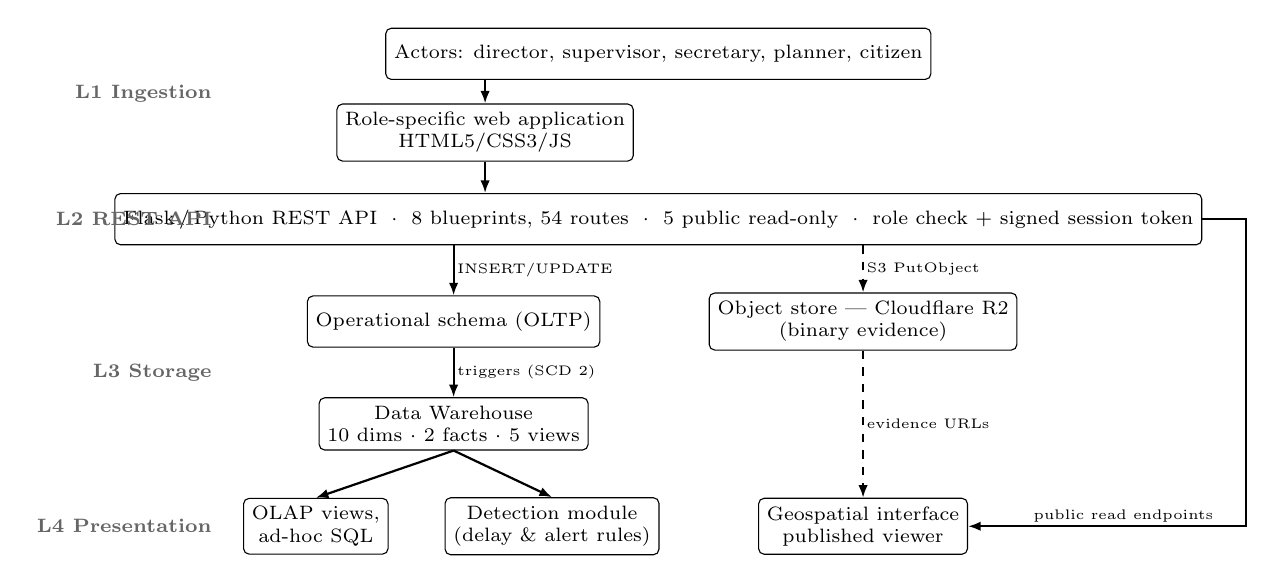
\begin{tikzpicture}[
  font=\scriptsize,
  box/.style={draw,rounded corners=2pt,align=center,minimum height=6.5mm,
              inner sep=3pt,fill=white,text=black},
  lay/.style={align=right,font=\scriptsize\bfseries,text=black!60},
  flow/.style={-{Latex[length=1.6mm]},thick},
  bin/.style={-{Latex[length=1.6mm]},thick,dashed},
  lbl/.style={font=\tiny,inner sep=1pt,fill=white},
  transform shape]

% ---- nodes ------------------------------------------------------------
\node[box] (act) at (0,3.55) {Actors: director, supervisor, secretary, planner, citizen};
\node[box] (web) at (-2.2,2.55) {Role-specific web application\\HTML5/CSS3/JS};
\node[box,minimum width=98mm] (api) at (0,1.45)
  {Flask\,/\,Python REST API $\;\cdot\;$ 8 blueprints, 54 routes $\;\cdot\;$
   5 public read-only $\;\cdot\;$ role check + signed session token};
\node[box] (oltp) at (-2.6,0.15) {Operational schema (OLTP)};
\node[box] (r2)   at ( 2.6,0.15) {Object store --- Cloudflare R2\\(binary evidence)};
\node[box] (dw)   at (-2.6,-1.15){Data Warehouse\\10 dims $\cdot$ 2 facts $\cdot$ 5 views};
\node[box] (olap) at (-4.35,-2.45){OLAP views,\\ad-hoc SQL};
\node[box] (det)  at (-1.35,-2.45){Detection module\\(delay \& alert rules)};
\node[box] (map)  at ( 2.6,-2.45){Geospatial interface\\published viewer};

% ---- layer labels -----------------------------------------------------
\node[lay,anchor=east] at (-5.55,3.05) {L1 Ingestion};
\node[lay,anchor=east] at (-5.55,1.45) {L2 REST API};
\node[lay,anchor=east] at (-5.55,-0.50){L3 Storage};
\node[lay,anchor=east] at (-5.55,-2.45){L4 Presentation};

% ---- edges ------------------------------------------------------------
\draw[flow] (act.south -| web) -- (web);
\draw[flow] (web) -- (web |- api.north);
\draw[flow] (api.south -| oltp) -- (oltp)
      node[lbl,midway,right] {INSERT/UPDATE};
\draw[bin]  (api.south -| r2) -- (r2)
      node[lbl,midway,right] {S3 PutObject};
\draw[flow] (oltp) -- (dw) node[lbl,midway,right] {triggers (SCD 2)};
\draw[flow] (dw.south) -- (olap.north);
\draw[flow] (dw.south) -- (det.north);
\draw[bin]  (r2) -- (map) node[lbl,midway,right] {evidence URLs};
\draw[flow] (api.east) -- ++(0.55,0) |- (map.east)
      node[lbl,pos=0.72,above] {public read endpoints};
\end{tikzpicture}}
\caption{System architecture (warehouse-centric), redrawn in English. The four
layers L1--L4 correspond to Sections~\ref{sec:l1}--\ref{sec:l4}. Solid arrows: structured-data
flow; dashed arrows: unstructured (binary) evidence flow. Released role-specific
pages read operational endpoints; the warehouse serves detection and OLAP through
	exttt{/api/analitica}. The geospatial viewer is part of the released artefact.}
\label{fig:arquitectura}
\end{figure}

\subsection{Layer 1: Ingestion}
\label{sec:l1}
The actors (directors, supervisors, secretaries, planners and registered citizens) interact with a web application built in HTML5/CSS3/JavaScript. Forms send structured data to the API (text, coordinates, amounts) and binary files (JPG/PNG, PDF) to the same endpoint, which routes them to their destination through an atomic transaction.

\subsection{Layer 2: REST API}
\label{sec:l2}
\begingroup
A Flask/Python REST API organised in eight blueprints exposes 54 routes, of which five are public and read-only (\texttt{/api/public/obras}, \texttt{/api/public/re\-gio\-nes}, \texttt{/api/public/resumen} and two evidence-listing routes). Access control for municipal staff is performed by a \texttt{@require\_auth} decorator that validates a role identifier transmitted in request headers; the participatory-budget module for citizens uses HMAC-signed session tokens issued with \texttt{itsdangerous} over the application secret. Passwords are stored as PBKDF2-HMAC-SHA256 hashes with a 16-byte random salt. We describe the scheme precisely because it is deliberately lightweight and is \emph{not} equivalent to a full token-based authentication service: hardening it (token expiry, rotation, and moving the staff role check from a header to a signed token) is listed among the limitations in Section~\ref{sec:limitaciones}.
\endgroup

\subsection{Layer 3: Storage}
\label{sec:l3}

\subsubsection{Object store (Cloudflare R2).}
An S3-compatible object store that receives unstructured evidence through direct ingestion. Paths follow a \textit{hive-partitioned} convention, shown in Equation~\eqref{eq:ruta-lake}:
\begin{equation}
\small\texttt{works/\{work\_id\}/reports/\{year\}-\{month\}/\{ts\}\_\{slug\}.\{ext\}}
\label{eq:ruta-lake}
\end{equation}
This structure enables direct exploration by work and period; each object's metadata (public URL, original name, MIME type, size in bytes, upload date) is also persisted in a warehouse-side table, creating a bidirectional link between the two layers.

\subsubsection{Data Warehouse (PostgreSQL/Supabase).}
An analytical layer with a star schema, two fact tables, and ten dimensions (Section~\ref{sec:warehouse}). The warehouse is populated from the operational schema by database triggers rather than by an external ETL job: eight triggers synchronise the dimensions (applying SCD~2 versioning where required) and four triggers emit rows into the audit fact table when a progress report, a cost record, an image upload or a citizen vote is registered. The warehouse uses range partitioning by year on the audit fact table to optimize historical queries.

\subsection{Layer 4: Presentation}
\label{sec:l4}
The released presentation layer consists of role-specific HTML/CSS/JavaScript pages that consume the REST API. Analytical consumption ---the five views of Section~\ref{sec:vistas}, ad-hoc OLAP queries and the detection module of Section~\ref{sec:modulo-deteccion}--- is served directly from the warehouse. The geospatial viewer of Figure~\ref{fig:mapa_interfaz} is published alongside the rest of the artefact and reads a frozen projection of the same synthetic dataset, so map and workspaces never disagree.

\subsection{Analytical Detection Module}
\label{sec:modulo-deteccion}
\begingroup
The component evaluated in Section~\ref{sec:eval-deteccion} is a stateless component that reads the warehouse and emits two artefacts: a \emph{delay set}, from \texttt{v\_delayed\_works}, containing every work whose latest monthly fact row carries the delay flag together with its slippage; and an \emph{alert stream}, from \texttt{v\_audit\_alerts}, which classifies audit events into five categories through a \texttt{CASE} expression over the fact table joined with the time, event-type and work dimensions.

The rule applied to a work--period record flags it as anomalous if \emph{any} of three operational criteria holds:
\begin{enumerate}
\item[C1.] \emph{Cost outlier}: the executed budget deviates from the mean by more than three standard deviations, $|b_i-\mu_b|/\sigma_b > 3$.
\item[C2.] \emph{Extreme delay}: the recorded slippage exceeds 120 days.
\item[C3.] \emph{Progress inconsistency}: physical progress below 30\% together with financial progress above 80\%.
\end{enumerate}
The corresponding anomaly score is $s_i=\max\left(\frac{|b_i-\mu_b|}{\sigma_b},\ \frac{d_i}{120}\mathbb{1}[d_i>120],\ 3.5\cdot\mathbb{1}[\text{C3}]\right)$, where $d_i$ is the slippage in days; the module flags $s_i>3$. The score is used for the ranking-based metrics reported in Section~\ref{sec:eval-deteccion}. C1--C3 are implemented as \texttt{v\_anomalies\_detection} over the monthly fact table and served read-only at \texttt{/api/analitica/anomalias}, so the rule evaluated in Section~\ref{sec:eval-deteccion} is the rule an operator runs. Until this revision they were different objects: the criteria lived only in the evaluation script and the snapshot left the columns C3 reads at \texttt{NULL}.
\endgroup

\subsection{A Note on Identifiers}
\label{sec:naming}
\begingroup
This article uses English identifiers for tables, columns and views; the published implementation uses Spanish ones, as it was built with and for a Spanish-speaking municipal office. The correspondence is mechanical ---\texttt{fact\_audit\_events} is \texttt{fact\_eventos\_auditoria}, \texttt{v\_delayed\_works} is \texttt{v\_obras\_retraso}, \texttt{dim\_work} is \texttt{dim\_obra}, and so on--- and the repository README tabulates every pair, so that a reader inspecting the code can locate each object referenced here. This mapping is a prerequisite for the reproducibility claims of Section~\ref{sec:resultados}.
\endgroup

% =====================================================================
\section{Data Warehouse Design}
\label{sec:warehouse}

The warehouse adopts a dimensional star model~\cite{Kimball2013} with two fact tables and ten dimensions, shown in Figure~\ref{fig:esquema_warehouse} with the SCD type of each.


\begin{figure}[htbp]
\centering

\resizebox{0.86\textwidth}{!}{%
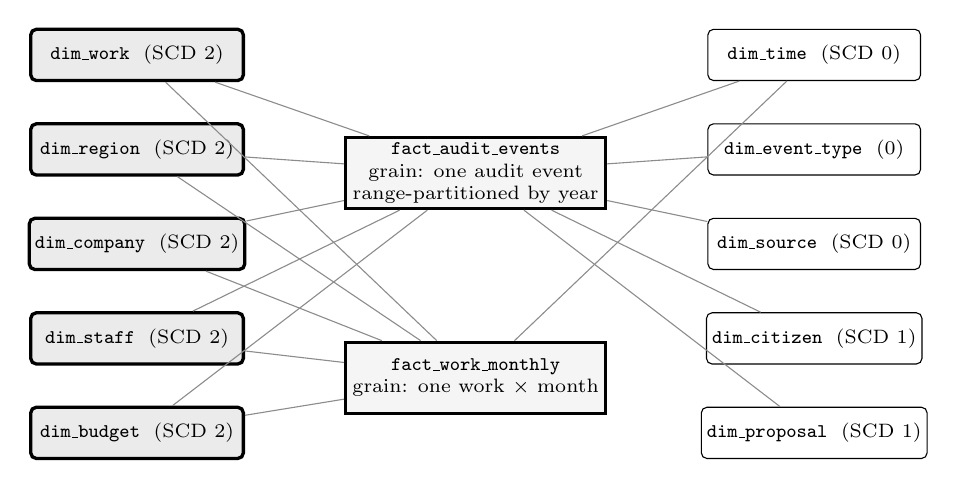
\begin{tikzpicture}[
  font=\scriptsize,
  d/.style={draw,rounded corners=2pt,align=center,minimum width=27mm,
            minimum height=6.5mm,inner sep=2pt,fill=white,text=black},
  d2/.style={d,fill=black!8,very thick},
  f/.style={draw,very thick,align=center,minimum width=33mm,
            minimum height=9mm,inner sep=2pt,fill=black!4,text=black},
  l/.style={draw=black!45,-},
  scale=1,transform shape]

% SCD 2 dimensions (left)
\node[d2] (w)  at (-4.3, 2.6) {\texttt{dim\_work} \;(SCD 2)};
\node[d2] (r)  at (-4.3, 1.4) {\texttt{dim\_region} \;(SCD 2)};
\node[d2] (c)  at (-4.3, 0.2) {\texttt{dim\_company} \;(SCD 2)};
\node[d2] (s)  at (-4.3,-1.0) {\texttt{dim\_staff} \;(SCD 2)};
\node[d2] (b)  at (-4.3,-2.2) {\texttt{dim\_budget} \;(SCD 2)};

% SCD 0/1 dimensions (right)
\node[d] (t)   at ( 4.3, 2.6) {\texttt{dim\_time} \;(SCD 0)};
\node[d] (et)  at ( 4.3, 1.4) {\texttt{dim\_event\_type} \;(0)};
\node[d] (so)  at ( 4.3, 0.2) {\texttt{dim\_source} \;(SCD 0)};
\node[d] (ci)  at ( 4.3,-1.0) {\texttt{dim\_citizen} \;(SCD 1)};
\node[d] (pr)  at ( 4.3,-2.2) {\texttt{dim\_proposal} \;(SCD 1)};

% facts
\node[f] (fa) at (0,1.1) {\texttt{fact\_audit\_events}\\\scriptsize grain: one audit event\\\scriptsize range-partitioned by year};
\node[f] (fm) at (0,-1.5) {\texttt{fact\_work\_monthly}\\\scriptsize grain: one work $\times$ month};

\foreach \n in {w,r,c,s,b} { \draw[l] (\n) -- (fa); }
\foreach \n in {t,et,so,ci,pr} { \draw[l] (\n) -- (fa); }
\foreach \n in {w,r,c,s,b} { \draw[l] (\n) -- (fm); }
\draw[l] (t) -- (fm);
\end{tikzpicture}}
\caption{Dimensional star schema, redrawn for legibility. Two fact tables
(\texttt{fact\_audit\_events}, range-partitioned by year, and
\texttt{fact\_work\_monthly}) are connected to the ten dimensions through
surrogate keys. The five Slowly Changing Dimensions of Type~2 (shaded, left)
are those that carry the historical traceability of the works. The monthly fact
table is conformed only with the five SCD~2 dimensions and the time dimension.}
\label{fig:esquema_warehouse}
\end{figure}

\subsection{Fact Tables and Grain}
\label{sec:grano}

We state the grain of each fact table explicitly, since it determines every subsequent aggregation and is a prerequisite for reproducing the design.

\textbf{\texttt{fact\_audit\_events}} has a grain of \emph{one row per audit event}: a single, atomic, immutable action performed on a work by an identified actor at an identified instant. It records events classified into 17 types (work creation, work modification, state change, progress report, cost record, budget record, budget modification, image upload, permit issue, hand-over record, contractor selection, funding assignment, supervisor assignment, role change, proposal registration, vote cast and session start) and is partitioned by year. The seeded scenario writes 8,934 events directly; the synchronisation triggers emit more as reports, costs, images and votes are registered, so a populated instance holds about 28,000. Each row carries foreign keys to the ten dimensions, financial metrics, progress metrics, and audit flags.

\textbf{\texttt{fact\_work\_monthly}} has a grain of \emph{one row per work per calendar month}. It is a periodic snapshot table: for each work and month it stores the total budget, the accumulated cost, the remaining balance, the percentage executed, the physical progress, the number of reports and images registered, and a boolean delay flag with the associated slippage in days. Because the grain is a snapshot rather than a transaction, aggregating cost across months requires taking the last snapshot of the period rather than a sum; the analytical views encapsulate this rule so that consumers cannot get it wrong.

\subsection{Slowly Changing Dimensions}
\label{sec:scd}

The SCD~2 dimensions~\cite{Kimball2013} (five in total: works, regions, companies, staff, and budget) maintain history through validity columns (\texttt{effective\_date}, \texttt{expiration\_date}, \texttt{is\_current}), which makes it possible to reconstruct the exact state of any work at an arbitrary point in time.

\begingroup
Three representative use cases motivate this choice, none answerable with a Type~1 dimension. In a \emph{budget-modification audit}, \texttt{dim\_budget} closes the current version and opens a new one, so an auditor can ask which amount was in force on the date a payment was authorised, not merely the amount in force today. Under \emph{contractor reassignment}, \texttt{dim\_company} preserves both versions, so progress recorded before the change stays attributed to the original contractor ---a precondition for any performance analysis by contractor. Under \emph{territorial reorganisation}, where communities are merged or renamed, \texttt{dim\_region} versioning prevents a historical investment series from being silently rewritten.

The remaining five do not version. \texttt{dim\_time} and \texttt{dim\_event\_type} are fixed catalogues (Type~0). \texttt{dim\_source} is Type~1: it carries running totals of works financed and amount assigned, which are overwritten as they change. \texttt{dim\_citizen} and \texttt{dim\_proposal} are Type~1 because only their current state is analytically meaningful and, since they hold names and national identity codes, retaining superseded versions would create a personal-data liability with no analytical return. The distribution is five Type~2, three Type~1 and two Type~0. An earlier version reported 5/2/3 while the SQL implemented 7/1/2, versioning the citizen dimensions against the privacy argument just given; \texttt{scripts/verificar\_scd.py} now checks the schema against this classification.
\endgroup

\subsection{Analytical Views and Refresh Strategy}
\label{sec:vistas}

Five analytical views derived from the fact tables support analytical consumption: (1)~\textbf{\texttt{v\_delayed\_works}} (works with a schedule slip and days of delay); (2)~\textbf{\texttt{v\_audit\_alerts}} (alerts classified as HIGH\_AMOUNT, CANCELLED\_WORK, BUDGET\_CHANGE, LATE\_EVENT and REVIEW); (3)~\textbf{\texttt{v\_work\_traceability}} (full SCD~2 version history of a work); (4)~\textbf{\texttt{v\_citizen\_participation}} (votes and proposals by region); and (5)~\textbf{\texttt{v\_budget\_executed}} (accumulated budget execution by funding source).

\begingroup
These are standard SQL views rather than materialized ones. The choice is deliberate and determines the refresh strategy. At the volumes involved ---of the order of $10^4$ fact rows for 64,844 inhabitants--- the views execute in tens of milliseconds over the partitioned fact table, so materialisation would buy little while introducing a staleness window; and since alerts must be actionable the moment a supervisor uploads a report, a live view is semantically preferable, with no refresh job to schedule or to fail. Should the deployment scale to several municipalities, the migration path is to materialise the aggregation-heavy \texttt{v\_budget\_executed} and \texttt{v\_citizen\_participation} with \texttt{REFRESH MATERIALIZED VIEW CONCURRENTLY} after each nightly load, keeping the two alert-bearing views live.
\endgroup

% =====================================================================
\section{Object Storage Layer: Evidence Storage}
\label{sec:datalake}

The object layer uses Cloudflare R2, a service compatible with the Amazon S3 API, selected for its zero egress cost and reduced global latency. In its current state it functions as an object repository for binary evidence (images and PDFs) linked to the warehouse, and not as a queryable analytical lake: analytical queries are resolved in the Data Warehouse, not over R2. Adopting an open table format~\cite{Armbrust2020} that enables direct queries over the lake is proposed as future work (Section~\ref{sec:conclusiones}). The path design follows the \textit{hive-partitioned} convention~\cite{Palkar2021} of Equation~\eqref{eq:ruta-lake}.

Ingestion is direct from the web form: the supervisor attaches images or PDFs when creating a progress report; the API computes the object key, uploads it through the S3 SDK, records the metadata in the warehouse, and returns the public URL. This is not an atomic transaction across the two stores: object storage and PostgreSQL cannot enlist in one. The implementation compensates ---on a database failure it issues a best-effort delete of the objects just uploaded--- so a crash between the two steps can still leave an orphaned object. Reconciling them would need a sweep against the metadata table, which is not implemented.

% =====================================================================
\section{Geospatial Interface Prototype}
\label{sec:grafo}

The geospatial display is an \emph{implicit} graph at the interface level ---the relationships are derived from the foreign keys of the dimensional model--- and not a formal knowledge graph with an ontology or an RDF triple store; publishing the schema as a linked vocabulary is addressed in future work.

Figure~\ref{fig:mapa_interfaz} shows the main interface, with markers color-coded by the state of the work and the technical-card popup that displays physical and financial progress indicators when a node is selected. It is part of the released artefact, reachable from the navigation bar of every page. Each marker sits at the real coordinates of its community, resolved from OpenStreetMap, with a deterministic offset of at most 150~m so that two works in the same community do not overlap. The community is therefore real; the exact site within it is not surveyed.

\begin{figure}[htbp]
\centering
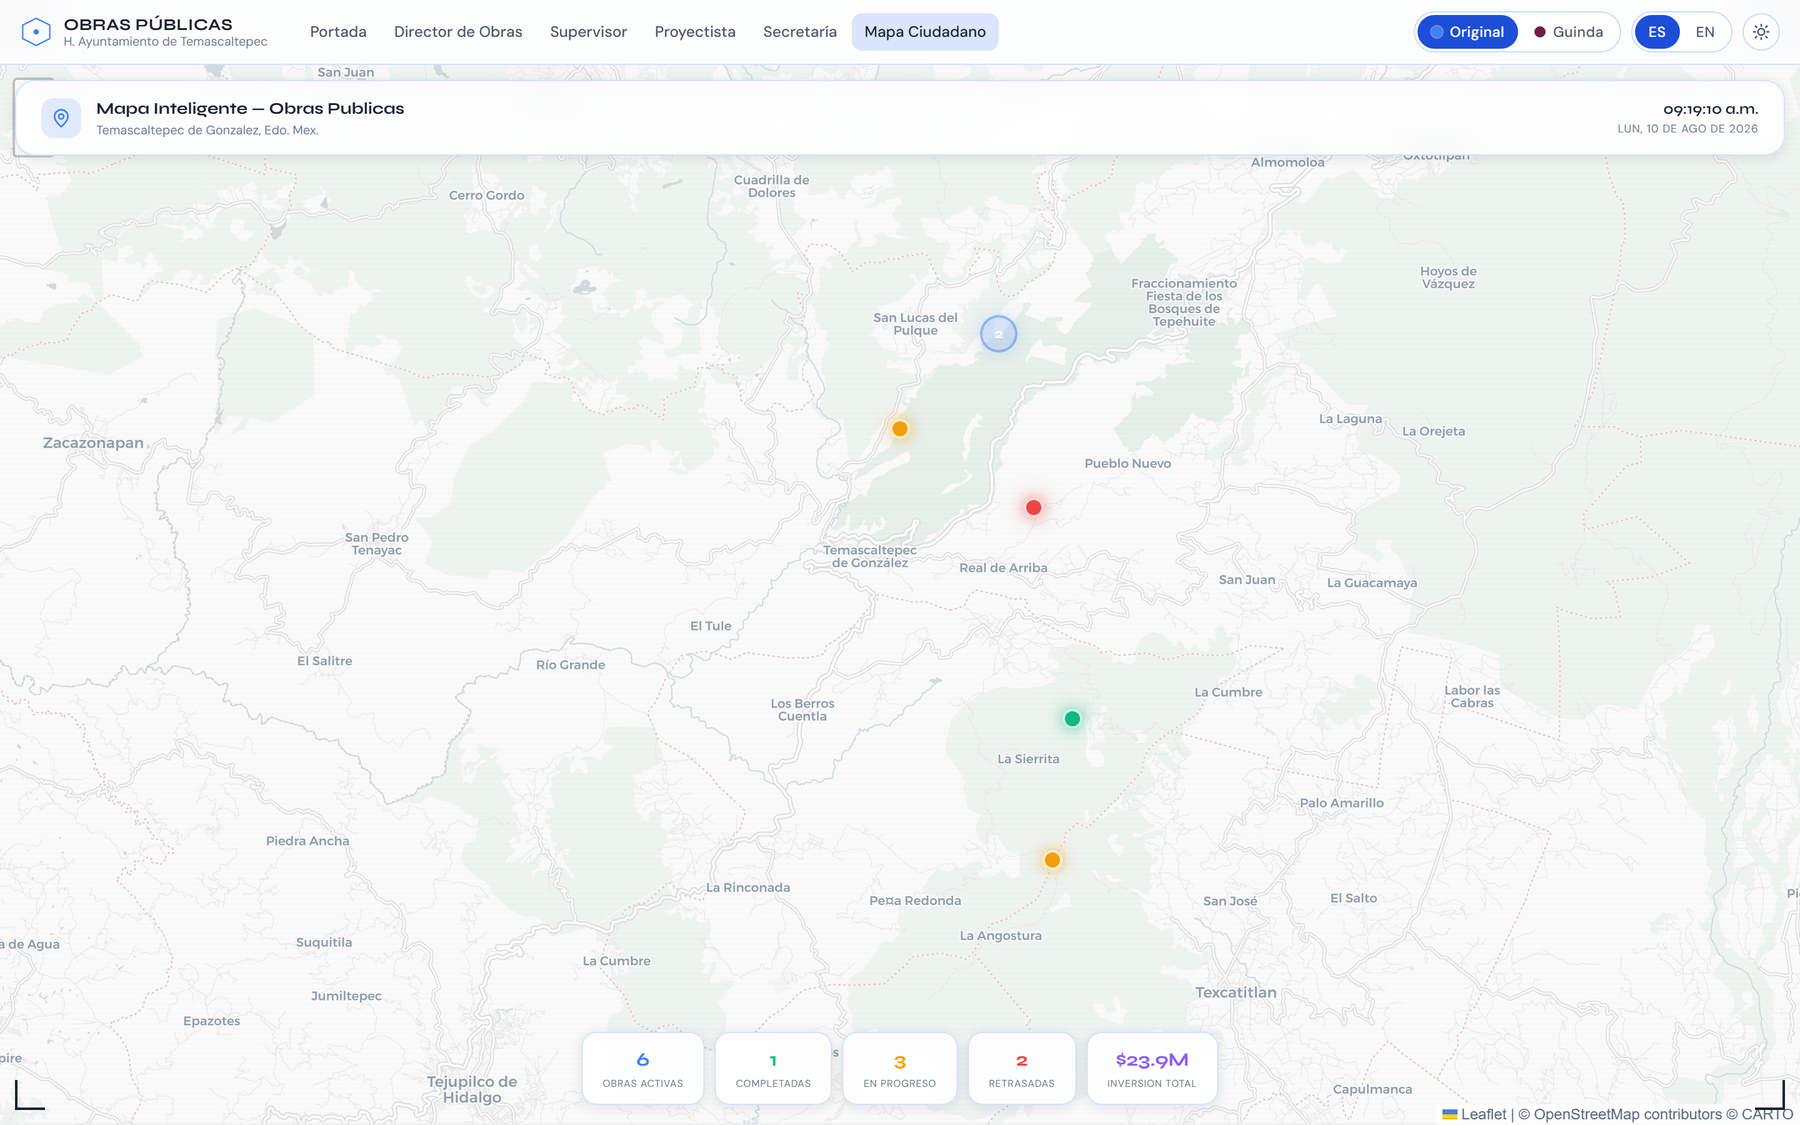
\includegraphics[width=0.74\textwidth]{mapa_publicado.png}
\caption{The published geospatial viewer, in light mode. Markers are color-coded by state ---green completed, amber in progress, red delayed--- over the six works of the demonstration dataset, with the indicator panel below. Live at {\small\url{https://gabrielhuav.github.io/PublicMunicipalWorks_DWH/mapa/?modo=claro}}, which reproduces this exact view.}
\label{fig:mapa_interfaz}
\end{figure}

\subsection{Management and Visualization Components}
\begin{itemize}
    \item \textbf{Marker layer:} each active work is represented by a marker color-coded by state ---green (completed), amber (in progress), red (delayed)--- derived from the work's latest progress report.
    \item \textbf{Technical card (popup):} selecting a work displays its file number, name, community, total budget, assigned company, date range, a physical-progress bar, and an expandable section for images from the object layer.
    \item \textbf{Analysis layer:} highlights delayed works and indicates the days of slippage (criterion C2 of Section~\ref{sec:modulo-deteccion}); the dual physical/financial percentage detects works with high budget execution and low physical progress (criterion C3), a potential indicator of irregularities.
\end{itemize}

% =====================================================================
\section{Results and Evaluation}
\label{sec:resultados}

\subsection{Scope of the Evaluation}
\label{sec:alcance}
\begingroup
Measured results and projections are kept strictly apart in what follows. The previous version also carried a third category, design targets; every figure in it has been either measured (Section~\ref{sec:objetivos}) or withdrawn. We label every figure in this section as \textbf{measured} (obtained by executing published code or auditing the published artefact, and reproducible by a third party: Sections~\ref{sec:objetivos}, \ref{sec:lighthouse} and~\ref{sec:eval-deteccion}) or \textbf{projected} (an expected operational outcome not yet observed in any deployment: Section~\ref{sec:impacto-social}). No number in this article is a measurement taken on real municipal data.

Three synthetic populations appear here and must not be conflated. The
\emph{published site} holds six works in the visitor's browser tab and supports
only interface claims and the delivery audit of Section~\ref{sec:lighthouse}.
The \emph{seeded warehouse} ---1,247 works, 55 communities, \$127.4~M, 29,928
monthly fact rows--- supports the structural claims and the latencies of
Section~\ref{sec:objetivos}. The \emph{detection dataset} is a separate
simulation of about 2,580 work--period records per seed and supports
Table~\ref{tab:eval-deteccion-anomalias} and nothing else.
\endgroup


\subsection{End-to-End Latency (Measured)}
\label{sec:objetivos}

The previous version of this chapter reported seven latency figures ---187~ms
on \texttt{/api/public/obras}, 1.42~s of map load, 543~ms for a gallery,
127~req/s sustained, 89~ms for the delayed-works view, 34~ms for an insert
firing the SCD~2 trigger and 112~ms of object-store read--- as design targets
derived from architectural sizing. No hardware, workload, repetition count or
raw output accompanied them, which makes them unfalsifiable. They are replaced
here by measurements taken against the stack in \texttt{docker/}, reproducible
with \texttt{scripts/medir\_rendimiento.py}.

\begin{table}[htbp]
\centering
\caption{Measured against the reference stack. API figures are 100 serial
requests over the seeded population (1,247 works); view figures are the server
execution time reported by \texttt{EXPLAIN ANALYZE} over 25 runs.}
\label{tab:latencias}
\scriptsize
\setlength{\tabcolsep}{4pt}
\renewcommand{\arraystretch}{1.1}
\begin{tabular}{l r r l}
\toprule
\textbf{Operation} & \textbf{Mean} & \textbf{p95} & \textbf{Previously claimed} \\
\midrule
\texttt{/api/public/obras} (753~kB)   & 566~ms & 610~ms & 187~ms \\
\texttt{/api/public/resumen}          & 544~ms & 589~ms & --- \\
\texttt{/api/public/regiones}         & 10.9~ms & 17.7~ms & --- \\
\texttt{/api/analitica/anomalias}     & 18.3~ms & 33.4~ms & --- \\
\texttt{v\_delayed\_works}            & 2.0~ms & 2.2~ms & 89~ms \\
\texttt{v\_anomalies\_detection}      & 23.8~ms & 24.5~ms & --- \\
\texttt{v\_budget\_executed}          & 5.2~ms & 5.4~ms & --- \\
Insert firing the SCD~2 trigger       & 0.1~ms & 0.1~ms & 34~ms \\
Sustained throughput (10 clients)     & \multicolumn{2}{c}{3.4~req/s} & 127~req/s \\
\bottomrule
\end{tabular}
\end{table}

Environment: Windows~10 host, Docker~29.6, PostgreSQL~16.14 in a container with
12 CPUs, Flask behind gunicorn with two synchronous workers, 1,247 works,
14,885 progress reports and 29,928 monthly fact rows.

The result answers RQ1 in a way the targets did not, and it does not flatter
the design uniformly. The warehouse is far quicker than claimed: the
delayed-works view runs in 2~ms against a claimed 89, and an insert firing the
SCD~2 synchroniser costs 0.1~ms against a claimed 34. The delivery layer is far
slower: \texttt{/api/public/obras} takes 566~ms against a claimed 187 because
it serialises the entire portfolio in one unpaginated response, and sustained
throughput is 3.4~req/s rather than 127 ---which is simply what two synchronous
workers and a 566~ms response give. Pagination and more workers are the
remedy, and neither touches the dimensional design. Reaching even these figures required removing a query-per-work pattern that
cost the two portfolio endpoints 7.5 and 12.5 seconds; the bottleneck was the
number of round trips, not PostgreSQL. Three of the original seven figures
---map load, gallery and object-store read--- are not reported: they need a
deployed map backend and an R2 bucket, and we prefer a gap to an unfalsifiable
number.

The seeded warehouse holds 1,247 works across 55 communities, 8,934 audit events, 3,421
photographic pieces of evidence, \$127.4~million pesos in budget, 2,156 citizen
proposals and 8,723 votes cast.

\subsection{Delivery of the Published Frontend (Measured)}
\label{sec:lighthouse}

The static artefact is permanently online, so its delivery can be audited by
anyone against a public URL. A Lighthouse audit of its two entry points, taken
as the median of three runs each on 11 August 2026 (Lighthouse 12.8.2, headless
Chrome 151, emulated mobile with simulated throttling, tag
\texttt{v1.5.0-icokg2026}), gives the landing page 85 for performance and the
map 72, with 100 for accessibility, 96 and 93 for best practices and 90 and 100
for SEO; both pages leave the main thread idle and shift no layout, and first
contentful paint is 3.2~s and 3.6~s. What separates them is delivery weight:
render-blocking fonts and a CDN animation library on one side, a 533~kB bundle
on the other. Reaching 100 on accessibility meant fixing what the audit
reported ---a brand link with no accessible name below 720~px, an attribution
painted below 4.5:1, two icon-only buttons, and map markers that are
\texttt{role="button"} elements with no text--- rather than restating the
score.

This audit measures the delivery of a static page. It executes no Flask, no
PostgreSQL and no warehouse query, so it is evidence about the front end alone;
the architecture is exercised in Section~\ref{sec:objetivos}.


\subsection{Evaluation of the Delay/Alert Detection Module (Measured)}
\label{sec:eval-deteccion}

\paragraph{What changed and why.} The protocol reported previously was
circular: three of its four injected classes were written as the detector's own
predicates, so their perfect recall was in the generator rather than measured.
Keeping the label in a column the detector never reads prevents leakage; it
does not make an evaluation non-circular.

\paragraph{Generator.} Anomalies are now latent states of a simulated execution
process, and what the detector sees are their observable consequences. A work
is drawn with a contract price, a planned duration and a productivity
parameter, and is then executed month by month under seasonal and remoteness
effects; payment follows progress with a mobilisation advance, a lag and noise.
Five latent causes are injected: a price inflated at award, an unproductive
contractor, payments running ahead of execution, a work that stops, and a work
contracted and paid but never built. Their magnitudes are drawn from
distributions that \emph{overlap the normal range}, so some anomalies are
undetectable in the recorded data and some healthy works look irregular. That
overlap is the condition for the evaluation to be informative.

\paragraph{Protocol.} Ten seeds and four latent prevalences (5, 10, 15 and
20\%); the main configuration is 15\%, which yields about 2,580 work--period
records per seed of which 17.2\% are anomalous. We report the mean over seeds
with a 95\% confidence interval. The baseline is an Isolation
Forest~\cite{Liu2008} (100 estimators, contamination set to the latent
prevalence) over five normalised features. Because comparing a rule at a fixed
threshold against a baseline at its default threshold compares two operating
points rather than two detectors, the baseline is also evaluated at a
\emph{matched alert budget}: the $k$ highest-scoring records, with $k$ the
number of alerts the rule raises.

\begin{table}[htbp]
\centering
\caption{Detection performance at 15\% latent prevalence. Mean over ten seeds
with a 95\% confidence interval; anomalies are latent process states, not
detector predicates. Reproducible with the published scripts.}
\label{tab:eval-deteccion-anomalias}
\scriptsize
\setlength{\tabcolsep}{4pt}
\renewcommand{\arraystretch}{1.15}
\begin{tabular}{l r r r r r}
\toprule
\textbf{Method} &
\multicolumn{1}{c}{\textbf{Precision}} &
\multicolumn{1}{c}{\textbf{Recall}} &
\multicolumn{1}{c}{\textbf{F1}} &
\multicolumn{1}{c}{\textbf{ROC-AUC}} &
\multicolumn{1}{c}{\textbf{PR-AUC}} \\
\midrule
Threshold rule (this work)        & $.463 \pm .056$ & $.352 \pm .031$ & $.398 \pm .038$ & $.628 \pm .022$ & $.307 \pm .053$ \\
Isolation Forest (default)        & $.369 \pm .053$ & $.321 \pm .031$ & $.342 \pm .037$ & $.650 \pm .029$ & $.342 \pm .052$ \\
Isolation Forest (matched budget) & $.387 \pm .054$ & $.295 \pm .033$ & $.333 \pm .039$ & $.650 \pm .029$ & $.342 \pm .052$ \\
\bottomrule
\end{tabular}
\end{table}

\paragraph{Results.} Table~\ref{tab:eval-deteccion-anomalias} is a much weaker
result than the one this chapter previously reported, and it is the one the
data supports. The rule alerts on about a third of the
anomalies and is right slightly less than half the time. It does not dominate
the baseline: Isolation Forest ranks better on both AUCs at every prevalence
tested, so as a scoring function the rule is the poorer of the two. Its
advantage is the operating point ---at the same alert budget it is more precise
(.463 against .387) and recovers more (.352 against .295)--- which matters
because an oversight office reviews a fixed number of files per period, not a
ranking. Both improve with prevalence (the rule from .219 to .556 precision
between 5 and 20\%).

\paragraph{Where it fails.} Per-cause recall is uneven in a way that is
diagnostic. The rule recovers unproductive contractors at $.548 \pm .059$,
ghost works at $.474 \pm .024$ and stopped works at $.388 \pm .011$, but
overpricing at only $.096 \pm .042$ and payments running ahead of execution at
$.061 \pm .034$. The reason is structural, not a matter of tuning. C1 compares an absolute
amount against a \emph{global} mean, so it flags large works rather than
overpriced ones: a school inflated by 30\% is still cheaper than an honest road.
And no criterion examines the \emph{gap} between physical and financial progress
unless the physical figure falls below 30\%, so a work paid steadily ahead of
its execution passes unremarked if it eventually finishes. The rule is a
schedule-failure filter with a narrow ghost-work check attached, not a
cost-anomaly detector, and this chapter no longer claims otherwise.

% =====================================================================

\section*{Declaration on the Use of Generative AI}

The authors used a generative AI assistant, under their direction, for language
editing, \LaTeX{} formatting, drafting text subsequently revised and approved by
the authors, and writing the auxiliary scripts distributed with the artefact, and generating the artefact's illustrative work images, each labelled as such in the file. The
research questions, the dimensional design, the ETL, the data collection, the
experiments and the interpretation of the results are the authors' own work.


\section*{Disclosure of Interests}
The authors declare that they have no conflicts of interest relevant to the content
of this article.

% =====================================================================
\begingroup\scriptsize\setlength{\parskip}{0pt}

\subsection{Illustrative Analytical Capability (Projected)}
\label{sec:impacto-social}

The warehouse answers questions a spreadsheet cannot: investment per
inhabitant by community against the development index, budget concentration
across funding sources, and participation rates by region. Over the seeded
population these queries return coherent, plausible figures, which shows the
analytical pipeline runs end to end. They are properties of the generator and
nothing else: no claim about territorial inequality, budget concentration or
savings in Temascaltepec is made or implied, and none can be until the model
is populated with municipal records.

% =====================================================================
\section{Conclusions and Future Work}
\label{sec:conclusiones}

\subsection{Conclusions}
This work presented a pragmatic architecture centered on a dimensional Data Warehouse for the geospatial monitoring of municipal public works, complementing the analytical store with S3-compatible object storage for unstructured evidence under a single REST API. Returning to the research questions: RQ1 is answered affirmatively at the design level ---ten dimensions, five of them SCD~2, two fact tables and five views on managed services at an estimated \$47~USD/month for 64,844 inhabitants--- with the caveat that no measurement on a stable production deployment exists yet. RQ2 is answered in Section~\ref{sec:warehouse}: an event-grain transaction fact table plus a work-month snapshot table, with SCD~2 restricted to the five audit-relevant entities, suffices to serve delay detection, budget alerting and participation analytics from one schema. RQ3 is answered in Section~\ref{sec:eval-deteccion}: the rule attains $0.46$ precision at $0.35$ recall against latent causes and is out-ranked by an unsupervised baseline, with its failures concentrated in cost anomalies, whose criterion is mis-specified.

The proposal shows that it is possible to build a transparency system with analytical capability (OLAP views, SCD~2 history), georeferenced photographic evidence, and citizen participation, without relying on high-cost enterprise platforms.

\subsection{Limitations}
\label{sec:limitaciones}
(1)~There is no hosted dynamic deployment: permanence rests on the static artefact, and the API is distributed to be run by whoever needs it rather than kept online by us. (2)~The participation module uses a simple voting scheme that may not adequately represent minorities. (3)~The quality of the analysis depends on the quality, coverage, and freshness of the data entered by field supervisors. (4)~All analytical results come from synthetic data (Faker, seed~42), due to privacy constraints on the open publication of municipal data; no result in this article has been validated against real municipal records. (5)~The architecture is, in its current state, \emph{data-warehouse-centric}: the object store holds binary evidence but is not queried analytically. (6)~The public map endpoints read the operational schema rather than the warehouse views, so the two read paths can diverge; unifying them is pending. (7)~Access control is lightweight ---the staff role travels in a request header and the citizen session token, though HMAC-signed, has no expiry--- which is adequate for a prototype whose analytical surface is public by design, but must be hardened before handling non-public data.

\subsection{Future Work}
(0)~Evolve the object layer toward a full lakehouse by adopting an open table format~\cite{Armbrust2020} (Apache Iceberg, or Parquet with transactional metadata) queryable directly over R2 through a lightweight engine such as DuckDB or Trino, without introducing Apache Spark; (1)~a computer-vision inference pipeline to automatically classify work progress from the stored photographs; (2)~publishing the schema as an OWL vocabulary to interoperate with Linked Data, and exposing an OC4IDS-conformant~\cite{OC4IDS} projection of the warehouse so that the municipality's data becomes comparable with other CoST-aligned jurisdictions; (3)~quadratic voting to improve the representativeness of minority proposals; (4)~time-series models to predict completion dates; (5)~recomputing the cost-anomaly criterion per work type, following the failure analysis of Section~\ref{sec:eval-deteccion}, and re-evaluating against the same ground truth; and (6)~validating the architecture in 3--5 additional municipalities of the State of Mexico, with a pre/post measurement of report-preparation time and information-request volume.

\subsection{Availability}
\label{sec:disponibilidad}
\begingroup
The warehouse DDL, SCD~2 triggers, seeded generators, load-testing scripts and the evaluation script are archived at {\small\url{https://github.com/gabrielhuav/PublicMunicipalWorks_DWH}}. A static demonstration is published through GitHub Pages at {\small\url{https://gabrielhuav.github.io/PublicMunicipalWorks_DWH/}}. It preserves the interface of the original public-works prototype---its four role workspaces, the citizen-participation module and the map---replacing remote authentication and writes with synthetic in-browser behaviour, and adds Spanish/English switching and two colour themes in light and dark mode. It therefore makes no request to any backend service. Access is open by construction: the credentials are printed on the landing page and the form accepts any value, even none; every screen is served from a synthetic dataset held in the visitor's own tab, so no input can affect another visitor. The Flask implementation in \texttt{backend/} remains the operational reference, where the same \texttt{DEMO-} accounts are constrained to read-only access. It is runnable, not archived: \texttt{docker/} raises PostgreSQL and the API with the warehouse and its seeded population, so an agency wanting to operate the system starts from a working stack; the figures above were verified against that container. Table~\ref{tab:eval-deteccion-anomalias} is reproduced by running \texttt{generar\_dataset\_obras.py} and \texttt{eval\_deteccion\_v2.py} from \texttt{scripts/evaluacion/}, both with seed 42. The population figures are constants in \texttt{scripts/generate\_synthetic\_data.py}, met by construction; its \texttt{-{}-verificar} flag checks them without a database.
\endgroup

% =====================================================================

\section*{Declaration on the Use of Generative AI}

The authors used a generative AI assistant, under their direction, for language
editing, \LaTeX{} formatting, drafting text subsequently revised and approved by
the authors, and writing the auxiliary scripts distributed with the artefact, and generating the artefact's illustrative work images, each labelled as such in the file. The
research questions, the dimensional design, the ETL, the data collection, the
experiments and the interpretation of the results are the authors' own work.


\section*{Disclosure of Interests}
The authors declare that they have no conflicts of interest relevant to the content
of this article.

% =====================================================================
\begingroup\scriptsize\setlength{\parskip}{0pt}
\begin{thebibliography}{16}

\bibitem{Zaharia2021}
Zaharia, M., et al.: Lakehouse: a new generation of open platforms that unify data warehousing and advanced analytics. In: Proceedings of the 11th Conference on Innovative Data Systems Research (CIDR 2021). Online (2021)

\bibitem{Kimball2013}
Kimball, R., Ross, M.: The Data Warehouse Toolkit: The Definitive Guide to Dimensional Modeling, 3rd edn. Wiley, Indianapolis (2013)

\bibitem{Palkar2021}
Palkar, S., Thusoo, A., Boncz, P.A.: Building a geospatial lakehouse, part 1. Databricks Engineering Blog (2021). \url{https://www.databricks.com/blog/2021/12/17/building-a-geospatial-lakehouse-part-1.html}. Last accessed 15 Jan 2026

\bibitem{Hogan2021}
Hogan, A., et al.: Knowledge graphs. ACM Comput. Surv. \textbf{54}(4), Article 71 (2021). \url{https://doi.org/10.1145/3447772}

\bibitem{Janowicz2022}
Janowicz, K., et al.: Know, know where, KnowWhereGraph: a densely connected, cross-domain knowledge graph and geo-enrichment service stack for applications in environmental intelligence. AI Mag. \textbf{43}(1), 30--39 (2022). \url{https://doi.org/10.1002/aaai.12043}

\bibitem{Poveda2020}
Espinoza-Arias, P., Fern\'andez-Ruiz, M.J., Morl\'an-Plo, V., Notivol-Bezares, R., Corcho, O.: The Zaragoza's knowledge graph: open data to harness the city knowledge. Information \textbf{11}(3), 129 (2020). \url{https://doi.org/10.3390/info11030129}

\bibitem{Lourenco2015}
Louren\c{c}o, R.P.: An analysis of open government portals: a perspective of transparency for accountability. Gov. Inf. Q. \textbf{32}(3), 323--332 (2015). \url{https://doi.org/10.1016/j.giq.2015.05.006}

\bibitem{Rajabi2023}
Rajabi, E., Midha, R., de Souza, J.F.: Constructing a knowledge graph for open government data: the case of Nova Scotia disease datasets. J. Biomed. Semant. \textbf{14}, 4 (2023). \url{https://doi.org/10.1186/s13326-023-00284-w}

\bibitem{Armbrust2020}
Armbrust, M., et al.: Delta Lake: high-performance ACID table storage over cloud object stores. Proc. VLDB Endow. \textbf{13}(12), 3411--3424 (2020). \url{https://doi.org/10.14778/3415478.3415560}

\bibitem{OC4IDS}
Open Contracting Partnership, CoST --- the Infrastructure Transparency Initiative: Open Contracting for Infrastructure Data Standard (OC4IDS). \url{https://standard.open-contracting.org/infrastructure/latest/en/}. Last accessed 1 Aug 2026

\bibitem{Hurtado2026}
Villa Vargas, J.M., Hurtado Avil\'es, G., Climent Hern\'andez, J.A.: Cuando M\'exico tiembla: la historia contada por los datos. AZCATL Rev. Divulg. Cienc. Ing. Innov. \textbf{4}(6), 28--33 (2026). \url{https://doi.org/10.24275/AZC2026E1004}


\bibitem{Liu2008}
Liu, F.T., Ting, K.M., Zhou, Z.-H.: Isolation forest. In: Proceedings of the 8th IEEE International Conference on Data Mining (ICDM 2008), pp. 413--422. IEEE Computer Society, Pisa (2008). \url{https://doi.org/10.1109/ICDM.2008.17}

\bibitem{Rivest2005}
Rivest, S., B\'edard, Y., Proulx, M.-J., Nadeau, M., Hubert, F., Pastor, J.: SOLAP technology: merging business intelligence with geospatial technology for interactive spatio-temporal exploration and analysis of data. ISPRS J. Photogramm. Remote Sens. \textbf{60}(1), 17--33 (2005). \url{https://doi.org/10.1016/j.isprsjprs.2005.10.002}

\bibitem{Faisal2014}
Faisal, S., Sarwar, M.: Handling slowly changing dimensions in data warehouses. J. Syst. Softw. \textbf{94}, 151--160 (2014). \url{https://doi.org/10.1016/j.jss.2014.03.072}

\bibitem{Ambituuni2025}
Ambituuni, A.: Infrastructure transparency initiative and anticorruption in public infrastructure projects: a principal--agent perspective to the antecedents that enable (or hinder) the effectiveness of transparency. Eng. Constr. Archit. Manag. \textbf{33}(7), 5934--5957 (2025). \url{https://doi.org/10.1108/ECAM-02-2025-0273}

\bibitem{Fazekas2020}
Fazekas, M., Kocsis, G.: Uncovering high-level corruption: cross-national objective corruption risk indicators using public procurement data. Br. J. Polit. Sci. \textbf{50}(1), 155--164 (2020). \url{https://doi.org/10.1017/S0007123417000461}

\end{thebibliography}\endgroup

\end{document}
